\documentclass[11pt,a4paper]{article}

\usepackage{url}
\usepackage{graphicx}
\usepackage{listings}
\title{Serial Communication with Rsapberry Pi using Bluetooth Module and Xbee.}
\author{e-Yantra Team}
\date{\today}

\begin{document}
	\maketitle
	\newpage
	\tableofcontents
	\newpage
	\section{Objective}
	To study Serial communication of Raspberry Pi with other devices using Bluetooth Module(HC-05) and then by using 2 XBee modules.
	\section{Prerequisites}
	\begin{itemize}
		\item A basic knowledge of Serial Communication.
	\end{itemize}
	\section{Hardware Requirement}
	\begin{enumerate}
		\item Raspberry Pi (I will be using Version 2 Model-B)
		\item Adapter (To power up an R-pi)
		\item PC 
		\item Bluetooth Module(HC-05)
		\item 2 Xbee Modules
	\end{enumerate}
	\section{Software Requirement}
	\begin{enumerate}
		\item XCTU 
		\item Blueterm		
	\end{enumerate}
	\newpage
	\section{Theory and Description}
	The universal asynchronous receiver/transmitter (UART) takes bytes of data and transmits the individual bits in a sequential fashion. At the destination, a second UART re-assembles the bits into complete bytes. Each UART contains a shift register, which is the fundamental method of conversion between serial and parallel forms. Serial transmission of digital information (bits) through a single wire or other medium is less costly than parallel transmission through multiple wires.
	 Serial communication is the process of sending data one bit at a time, sequentially, over a communication channel.Asynchronous serial data communication is widely used for character-oriented transmissions, while block-oriented data transfers use the synchronous method. In the asynchronous method, each character is placed between start and stop bits. This is called framing. In data framing for asynchronous communications, the data, such as ASCII characters, are packed between a start bit and a stop bit. The start bit is always one bit, but the stop bit can be one or two bits. The start bit is always a 0 (low) and the stop bit(s) is 1 (high).For example, ASCII character “A” (8-bit binary 0100 0001) is framed between the start bit and a single stop bit. Notice that the LSB is sent out first.
	 \begin{figure}[h!]
	 	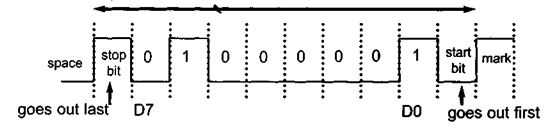
\includegraphics[width=10cm]{Asy_serial.JPG}
	 	\centering
	 	\caption{[3]}
	 \end{figure}
	 when there is no transfer, the signal is 1 (high), which is referred to as mark. The 0 (low) is referred to as space. Notice that the transmission begins with a start bit followed by DO, which is the LSB, then the rest of the bits until the MSB (D7), and finally, the one stop bit indicating the end of the character “A”.
	 The rate of data transfer in serial data communication is stated in bps (bits per second). Another widely used terminology for bps is baud rate.
	\subsection{Bluetooth Module HC-05:}
	HC-05 module is an easy to use Bluetooth SPP (Serial Port Protocol) module, designed for transparent wireless serial connection setup.
	\newline
	    \textbf{Hardware Specifications:}
		\begin{itemize}
			\item UART interface with programmable baud rate
			\item Vcc :to power the bluetooth module (It should be in the range of 3.3V to 6V)
			\item Ground pin
			\item RxD :connected to the TXD pin of Raspberry Pi(receives the data from Raspberry Pi)
			\item TXD :connected to the RXD pin of Rsapberry pi(transmits the data to raspberry pi which it receives from other connected device)
		\end{itemize}
		\begin{figure}[h!]
			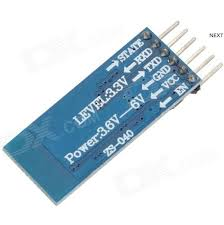
\includegraphics[width=10cm]{HC-05.jpg}
			\centering
			\caption{[3]}
		\end{figure}
	\subsection{XBee }
	Xbee can be used for wireless communication with low power consumption. A 3.6V 600mA Lithium battery may last 6 - 12 months for powering up an Xbee while the wireless range can up to 1 mile. It talks with well known UART interface and makes it easy to use. It is simple and straight forward if you only use 2 Xbee for communication. Xbee is the module using Zigbee protocol. Zigbee is a wireless communication protocol like wifi and bluetooth.  
		\begin{figure}[h!]
			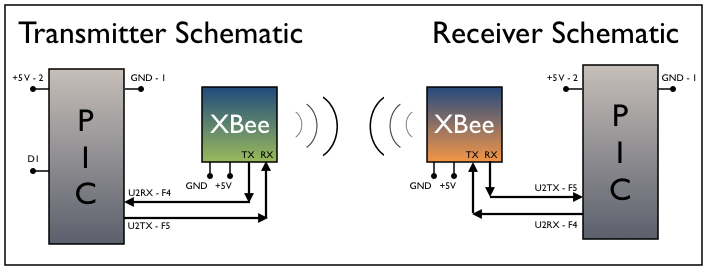
\includegraphics[width=10cm]{XBee.jpg}
			\centering
			\caption{[3]}
		\end{figure} 
	we have to just connect 4 pins of Xbee to raspberry pi which are:
	\begin{enumerate}
		\item pin 1(3.3V) to Raspberry Pi pin 1 which is 3.3V.
		\item pin 2(UART DATA OUT) to Rasberry Pi pin 10(UART\_RXD)
		\item pin 3(UART DATA IN) to Raspberry Pi pin 8(UART\_TXD)
		\item pin 10(Ground) to Raspberry Pi Ground
	\end{enumerate}
	\textbf{Pin Diagram of XBee:}
			\begin{figure}[h!]
				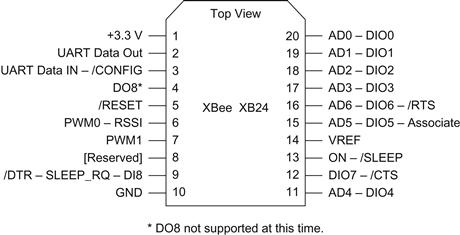
\includegraphics[width=10cm]{Xbee_pin_diag.jpg}
				\centering
				\caption{[3]}
			\end{figure} 
		\newpage
		
	\subsection{Enabling UART Communication on Raspberry Pi:}
	To make Raspberry Pi Compatible for Serial communication we need to follow the following steps:
	\begin{itemize}
		\item We have to make changes to the configuration file cmdline.txt
		\item Before making any changes to this configuration file, save the file in the case you make any mistake.
		\item File /boot/cmdline.txt contains the kernel options that are used to boot the system.
		\newline In the Terminal window type the command:
		\newline \textbf{sudo nano /boot/cmdline.txt}
		\item A window will open showing the following options:
		\newline \textbf{dwc\_otg.lpm\_enable=0 console=ttyAMA0,115200 console=tty1 root=/dev/mmcblk0p2 rootfstype=ext4 elevator=deadline rootwait}
		\newline The interesting option is console, because this configure the serial port device /dev/ttyAMA0 to 115200 bps.Remove this serial reference by taking away the option \textbf{console=ttyAMA0,115200 }. After you make these changes the file should read:
		\newline \textbf{dwc\_otg.lpm\_enable=0 console=tty1 root=/dev/mmcblk0p2 rootfstype=ext4 elevator=deadline rootwait}
		\item If you are using older version of Raspbian OS then you will find another option in the above mentioned line \newline \textbf{kgdboc=ttyAMA0,115200}
		\newline Just remove the option from cmdline.txt.
		\item Also there is another configuration file \textbf{/etc/inittab}. Just open the file and inside this file you have to locate the following line: 
		\newline \textbf{T0:23:respawn:/sbin/getty -L ttyAMA0 115200 vt100}
		\newline We will comment out the serial console task:
		\newline \textbf{\#T0:23:respawn:/sbin/getty -L ttyAMA0 115200 vt100}
		\item After making these changes reboot the system so that they take effect. With these changes the RPi will not use the serial port at all, so the port will be free to any application that wants to use it as /dev/ttyAMA0.
		\item If you want to play with sending and receiving data through the serial port then you can install minicom into your RPi using the following command:
		\newline \textbf{sudo apt-get install minicom}
		\newline And then you can open a terminal on the serial port with this command:
		\newline \textbf{minicom -b 9600 -o -D /dev/ttyAMA0}
		\newline Anything you type inside the minicom terminal will be sent to the serial port, and anything the other side sends will be displayed.
	\end{itemize}
	\flushleft
	\section{Experiment}
	\subsection{Communication between Rpi and Android device using HC-05 (Bluetooth Module):}
	\begin{itemize}
		\item Connect the pins of HC-05 to Raspberry Pi as shown in below figure:
		\begin{figure}[h!]
			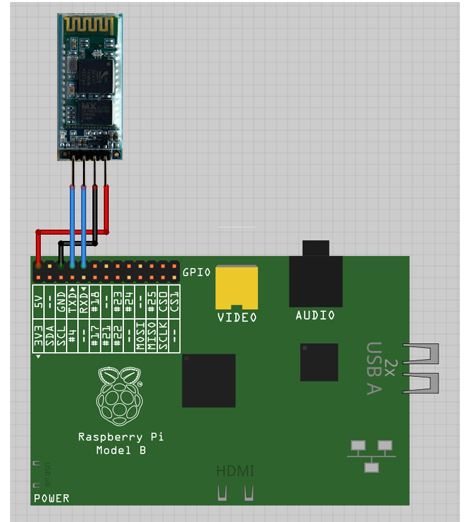
\includegraphics[width=10cm]{HC-05_connection.JPG}
			\centering
			\caption{[3]}
		\end{figure}
		\newpage 
		\begin{tabular}{|c|c|c|}
			\hline
			RPi GPIO pin & HC-05(bluetooth) module pin \\
			\hline 
			5V (Pin 2) & Vcc\\
			\hline
			GND (Pin 6) & GND\\
			\hline 
			TXD (Pin 8) & RXD\\
			\hline 
			RXD (Pin 10) & TXD\\
			\hline			
		\end{tabular}
		\flushleft
	\end{itemize}
	\begin{itemize}
		\item Configure the bluetooth module as the Bluetooth module comes preconfigured from the factory with a set of defaults, which are:
			\begin{enumerate}
			\item Baud rate: 9600
			\item Bluetooth ID: linvor
			\item PIN: 1234
			\end{enumerate}
		 If you want to change any of the above options then you can change them by using AT commands.
		\item Download the Blueterm app on your Android Device and connect to the HC-05 via bluetooth obviously.
		\item Now we will write a program in python to serially transmit and receive data as:
		\newline \textbf{CODE:}
		\newline 
		\vspace{0.3cm}
		
		\lstinputlisting[language=python]{Bluetooth.py}
		\newpage
		\item In the Blueterm app on your Android device you will see the data transmitted by Raspberry Pi through HC-05 as:
		\newline 
		\begin{figure}[h!]
			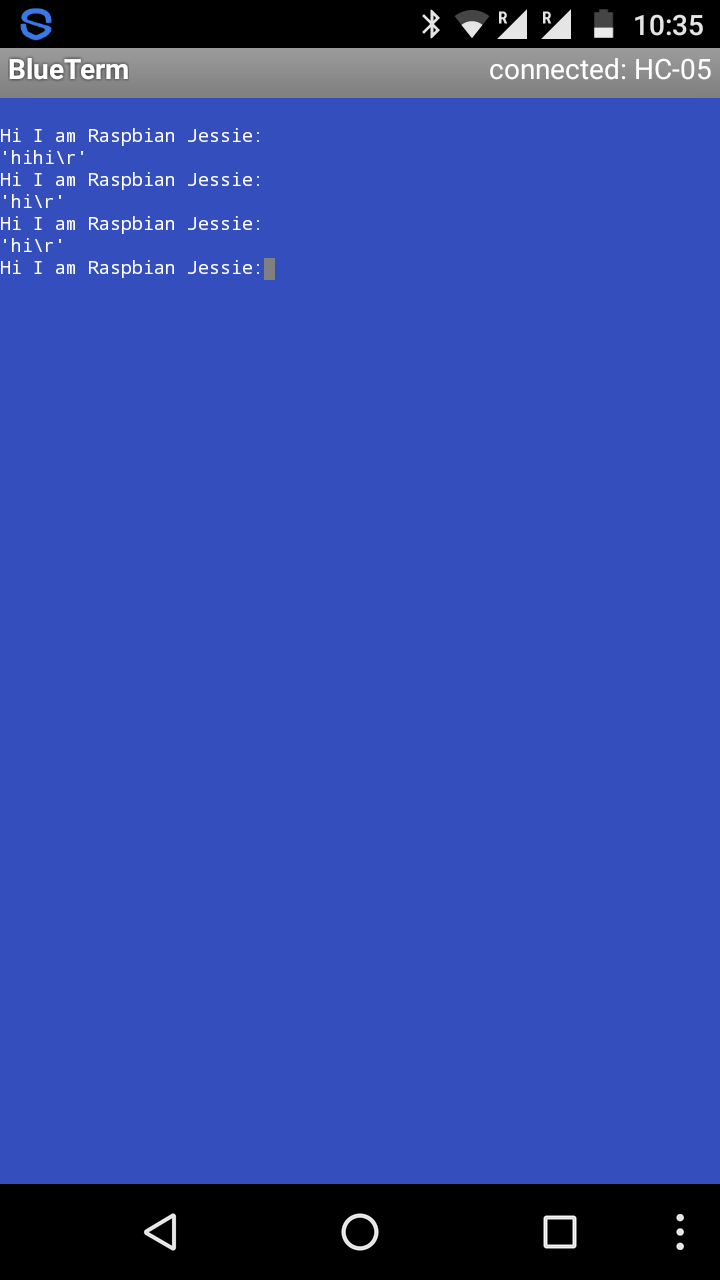
\includegraphics[width=10cm]{img_2.JPG}
			\centering
			\caption{[3]}
		\end{figure} 
		\newline
		\item The data transmitted by the device will be received by the bluetooth module serially, which will then sent the data to the raspberry pi.
		 \begin{figure}[h!]
		 	\includegraphics[width=10cm]{img_1.JPG}
		 	\centering
		 	\caption{[3]}
		 \end{figure}  
	\end{itemize}
	In this way the Data can be transmitted and received serially by the Raspberry Pi using Bluetooth module.
	
	\subsection{Communication between Rpi and PC using XBee Module:}
	\begin{itemize}
		\item First of all download XCTU software on your PC and open it.
		\begin{figure}[h!]
			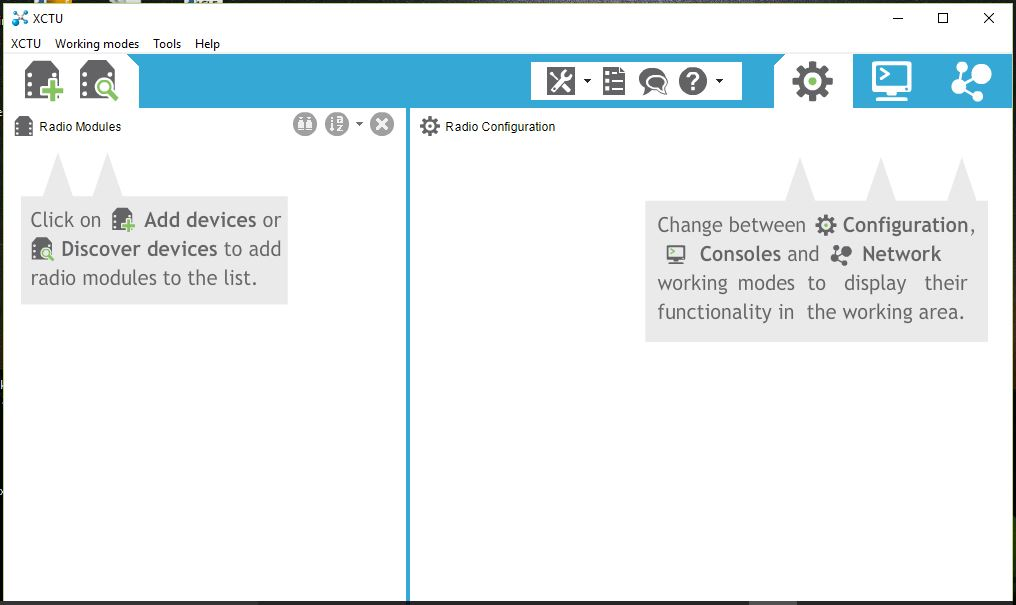
\includegraphics[width=10cm]{Capture1.jpg}
			\centering
			\caption{[3]}
		\end{figure} 
		\item Connect both the Xbee's to the PC one by one by USB jack(to configure Xbee's) and click on the Radio module on the extreme left of the window.A window named 'Add Radio Module' will occur on the screen select one Serial/USB port.
		\begin{figure}[h!]
			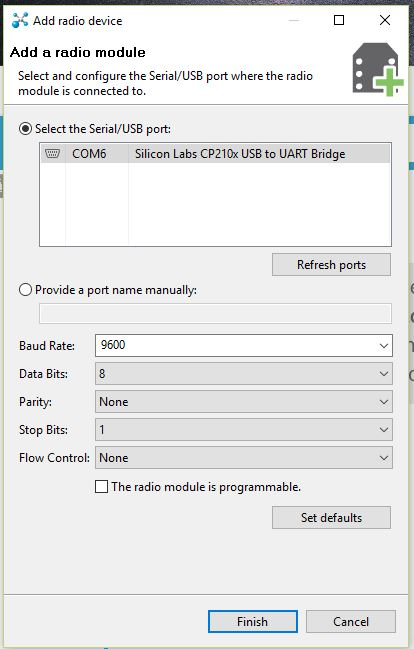
\includegraphics[width=10cm]{Capture2.jpg}
			\centering
			\caption{[3]}
		\end{figure} 
		\item On the left side of the window the radio module will be shown. Select the Radio module to display it's properties and configure it.
		\begin{figure}[h!]
			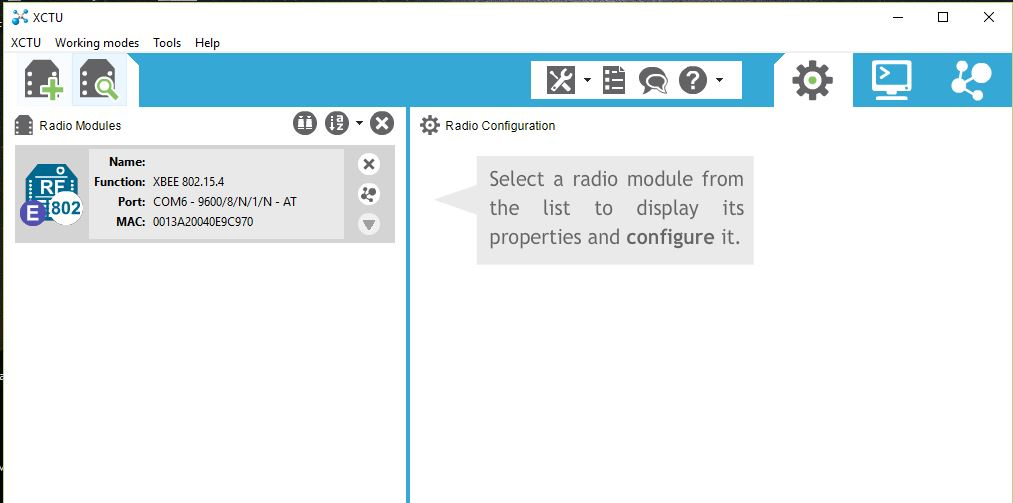
\includegraphics[width=10cm]{Capture3.jpg}
			\centering
			\caption{[3]}
		\end{figure} 
		\item Radio configuration window will open. First click on 'Default' to set all the parameters to default values.
		\begin{figure}[h!]
			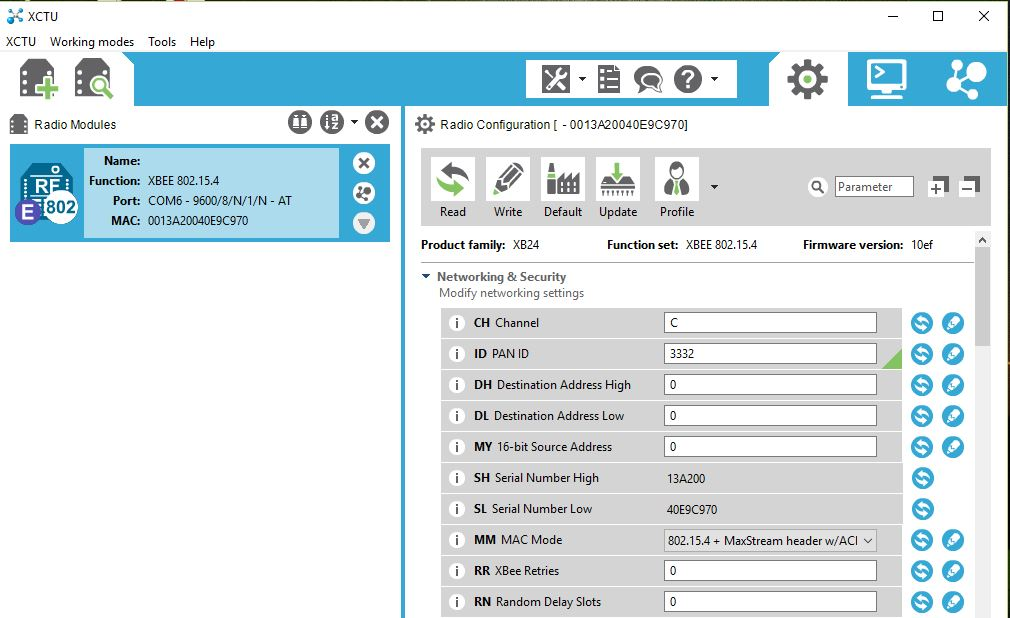
\includegraphics[width=10cm]{Capture4.jpg}
			\centering
			\caption{[3]}
		\end{figure} 
		\item Then change the PAN ID (if you want).
		\begin{figure}[h!]
			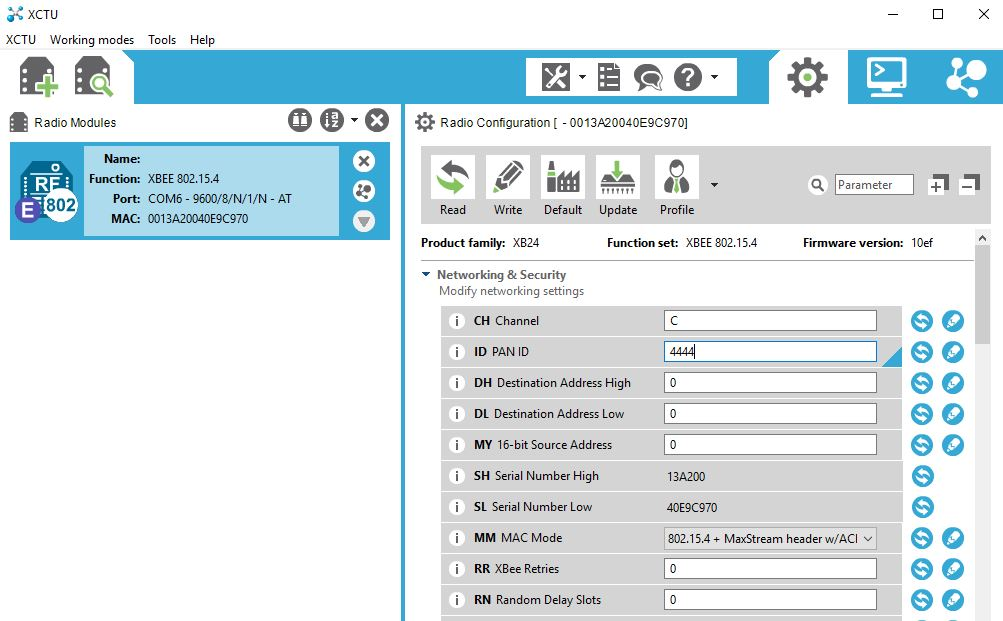
\includegraphics[width=8cm]{Capture5.jpg}
			\centering
			\caption{[3]}
		\end{figure}  
		\newpage
		\item Continue the same procedure with other XBee module also. Just keep in mind to set the PAN ID same as the first XBee module otherwise they will not communicate.
		\item Then disconnect one of the XBee from the PC and connect it to Raspberry Pi.
	\item 
	Make the connections of XBee to the Raspberry Pi as shown below:
	\begin{figure}[h!]
		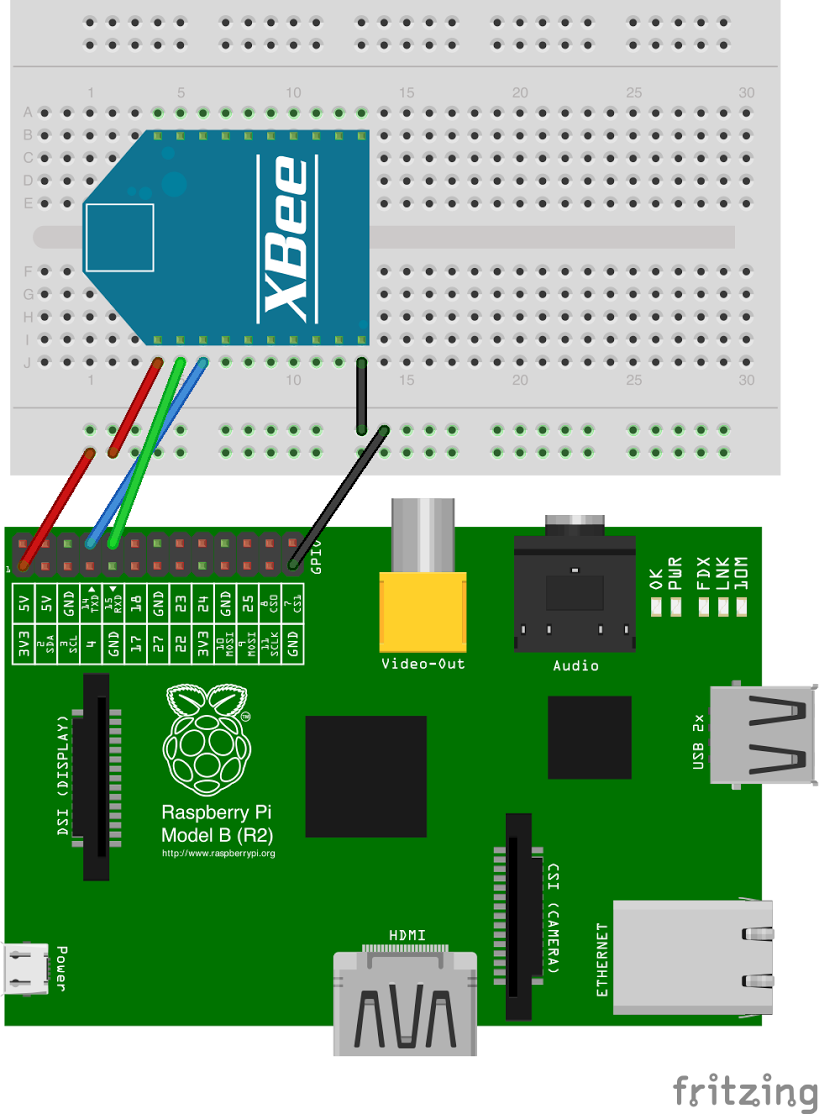
\includegraphics[width=7cm]{rasp_pi_to_xbee.jpg}
		\centering
		\caption{[3]}
	\end{figure} 
	\newpage
	 You can also directly use the USB jack to connect Xbee and Raspberry Pi.
	\item Run the same code as used for the BLuetooth module(HC-05).
	\item On the XCTU there is a option "close". This makes the connection between two XBee modules.
	\item The data transmitted by one XBee (connected to the RPi), will be received by second XBee serially and this will be shown on "Console Log" on XCTU as:
	\begin{figure}[h!]
		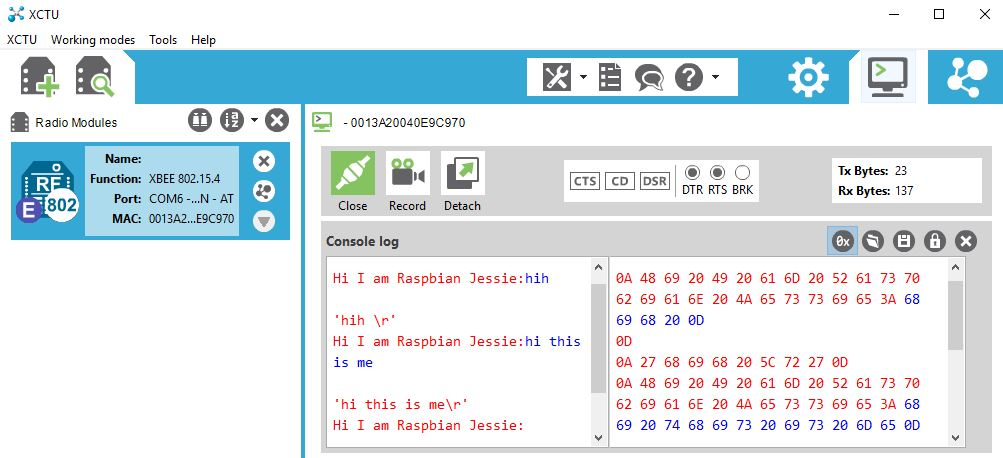
\includegraphics[width=10cm]{Capture6.jpg}
		\centering
		\caption{[3]}
	\end{figure} 
	\newpage 
	\item Similarly the data sent by second XBee will be transmitted serially to first XBee connected to RPi.The data sent is as:
	\begin{figure}[h!]
		\includegraphics[width=10cm]{img_3.jpg}
		\centering
		\caption{[3]}
	\end{figure} 
	\end{itemize}
	In this way the Data can be transmitted and received serially by the Rspberry Pi using Bluetooth module.
	\newline 
	\textbf{NOTE:} if you are using USB jack then use \textbf{/dev/ttyUSB0} as the device path in the above given program, otherwise if you are connecting to the serial GPIO pins of Raspberry Pi(RXD \& TXD) then use \textbf{/dev/ttyAMA0}
	\section{References}
		\begin{enumerate}
			\item \url{http://www.elinux.org/Serial_port_programming}
			\item \url{http://blog.miguelgrinberg.com/post/a-cheap-bluetooth-serial-port-for-your-raspberry-pi}
			\item \url{https://en.wikipedia.org/wiki/XBee}
		\end{enumerate}
\end{document}



